\section{FLiDASH: Federated Adaptive Bitrate Live Streaming over Locality Sensitive Playback Coalitions}
Live streaming is a unique service over the Internet that is an alternative to television (TV) broadcast yet more flexible. Few live streaming providers allow the ability to add custom delays in the live feed. However, the most popular live-streaming flavor is without any user-defined delays (i.e., live). The live stream has a unique property of synchronous playback by millions of players. In mega-events live streaming, we find another attractive property that many players belong to the same local networks. The players share a common network with two particular models, a) users have different plans, the network belongs to the Internet provider, b) the network belongs to the users, and they have a shared Internet connection. In this work, we aim to develop a DASH-based live streaming system where players form coalitions if connected via a local network and stream the live video as a group. In the case of a large network, Application-Layer Traffic Optimization (ALTO) server will be used to find appropriate players to form a coalition. Our goal is to improve quality for the entire coalition and ensure every player contributes to the common goal.

\subsection{Architecture}
FLiDASH system has three components: a) Streaming server: host the video data. b) Streaming client: plays the video. c) Proximity server: keep track of players. While the streaming server is an unmodified web server, the client is designed especially for FLiDASH live video streaming. It acts as a normal DASH-based player if there are no other players nearby. However, it continuously looks for nearby players to form a coalition. The proximity server helps a player to find nearby players. Before a coalition can be formed, clients first check whether they are compatible or not, primarily by the expected video quality level. Once a coalition is formed, the coalition based video streaming system starts, and video quality improves drastically.
\subsection{Adaptive streaming system}
As FLiDASH is a collaborative streaming system, we need to decide which player will download which segment and what will be the quality. Our aim to maximize quality by keeping every player busy\footnote{Here, a player is busy if it is downloading a segment from the CDN; otherwise, it is idle.} all the time. We achieve this goal by scheduling a segment to an idle player for maximum time or who has the least amount of data to be downloaded among busy players. Once the player is chosen, that player is informed to download the segment. Each player decides the segment quality based on its bandwidth, deadline to finish downloading, and other players' decisions about the previous segment. The chosen player also decides the next downloader and informs it. It is expected that the chosen player will be able to download the segment before it is required to play the stream without interruption. However, we have introduced a fail-safe mechanism if a designated player fails to download the segment before the deadline. More details are available in the thesis.

\subsection{Evaluation}
We have performed evaluations of FLiDASH on the emulated environment with two types of scenarios a) every player has their Internet connection, and b) players share a common internet connection. We have developed a prototype using {\tt python} and evaluated our system. We compare our system with modern ABR algorithm BOLA, MPC, and Pensieve and a system with a Distributed Hash Table (DHT). We compare the QoE of both the scenario in Fig.~\ref{fig:FLiDASH:QoE}, which supports our claim that collaboration improves the overall quality.
\begin{figure}[h]
	\captionsetup[subfigure]{width=0.49\linewidth}
	\begin{center}
		\subfloat[\label{fig:FLiDASH:ind_qoe}Indipendent Internet connection]{
			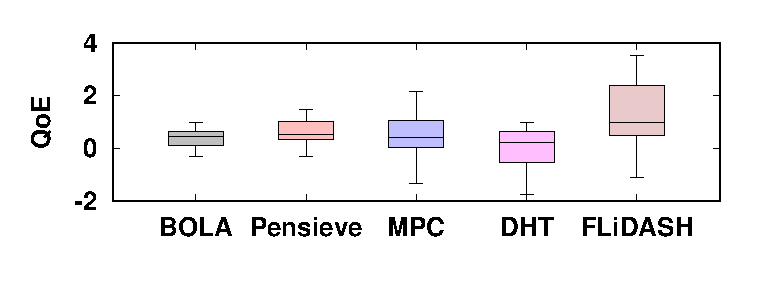
\includegraphics[width=0.49\linewidth]{img/FLiDASH/ind_qoe_box_1}
		}
		\subfloat[\label{fig:FLiDASH:shared_qoe}Shared Internet connection]{
			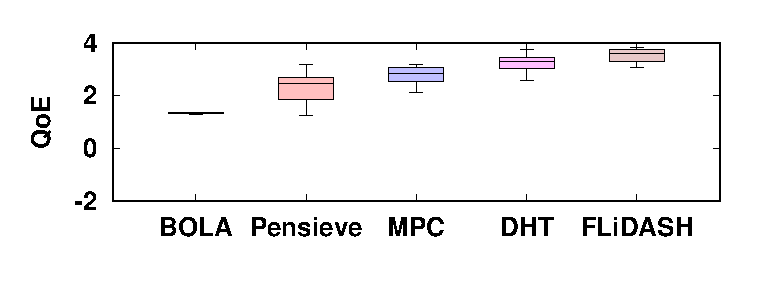
\includegraphics[width=0.49\linewidth]{img/FLiDASH/shared_qoe_box_1}
		}
	\end{center}
	\caption{\label{fig:FLiDASH:QoE}Comparison of video streaming system in terms of QoE}
\end{figure}
